\documentclass[12pt]{article}
% ===========================================================================
% preambulo-uis.tex
% Formato de trabajo de grado UIS, APA 7.
% Ver AGENTS.md, secciones 1 a 9. No cambiar valores de forma sin instruccion.
% ===========================================================================

% ---------- Codificacion, idioma y fuente ----------
\usepackage[utf8]{inputenc}
\usepackage[T1]{fontenc}
% es-tabla: "Tabla" en vez de "Cuadro".
% es-nosectiondot: sin punto tras numeros de seccion (se repone solo en nivel 1).
\usepackage[spanish,es-tabla,es-nosectiondot]{babel}
\usepackage{amsmath}               % antes de newtxmath
\usepackage{newtxtext}            % Times New Roman
\usepackage{newtxmath}            % incluye los simbolos de amssymb
\usepackage{csquotes}

% ---------- Pagina: carta, margenes 2,54 cm uniformes ----------
\usepackage[letterpaper,margin=2.54cm,headheight=15pt]{geometry}

% ---------- Interlineado doble, sangria 1,27 cm, justificado ----------
\usepackage{setspace}
\doublespacing
\setlength{\parindent}{1.27cm}
\setlength{\parskip}{0pt}

% ---------- Paquetes de contenido ----------
\usepackage{graphicx}
\graphicspath{{figuras/}}
\usepackage{booktabs}
\usepackage{array}
\usepackage{makecell}
\usepackage[table]{xcolor}
\usepackage{enumitem}
\setlist{nosep}
\usepackage{tikz}
\usetikzlibrary{arrows.meta,positioning,fit,backgrounds,babel}

\definecolor{morado1}{HTML}{7B6BAF}
\definecolor{azul2}{HTML}{A4C2F4}
\definecolor{verde1}{HTML}{76A5AF}
\definecolor{lima1}{HTML}{B6D7A8}

% ---------- Cornisa y paginacion ----------
% Cornisa: izquierda, MAYUSCULA SOSTENIDA, maximo 50 caracteres.
% Paginacion arabiga desde la portadilla (pagina 1).
\usepackage{fancyhdr}
\newcommand{\cornisa}{OPEN VOCABULARY CHANGE DETECTION} % 32 caracteres
\pagestyle{fancy}
\fancyhf{}
\fancyhead[L]{\cornisa}
\fancyhead[R]{\thepage}
\renewcommand{\headrulewidth}{0pt}
\fancypagestyle{plain}{%
  \fancyhf{}%
  \fancyhead[L]{\cornisa}%
  \fancyhead[R]{\thepage}%
  \renewcommand{\headrulewidth}{0pt}}

% ---------- Jerarquia de titulos (5 niveles APA) ----------
\usepackage{titlesec}
\setcounter{secnumdepth}{5}
% Nivel 1: centrado, negrita, punto tras el numero.
\titleformat{\section}[block]{\centering\bfseries\normalsize}{\thesection.}{0.5em}{}
\titlespacing*{\section}{0pt}{2\baselineskip}{2\baselineskip}
% Nivel 2: margen izquierdo, negrita.
\titleformat{\subsection}[block]{\bfseries\normalsize}{\thesubsection}{0.5em}{}
\titlespacing*{\subsection}{0pt}{\baselineskip}{\baselineskip}
% Nivel 3: margen izquierdo, negrita y cursiva.
\titleformat{\subsubsection}[block]{\bfseries\itshape\normalsize}{\thesubsubsection}{0.5em}{}
\titlespacing*{\subsubsection}{0pt}{\baselineskip}{\baselineskip}
% Nivel 4: con sangria, negrita, termina en punto, texto en la misma linea.
\titleformat{\paragraph}[runin]{\bfseries\normalsize}{\theparagraph}{0.5em}{}[.]
\titlespacing*{\paragraph}{1.27cm}{\baselineskip}{0.5em}
% Nivel 5: con sangria, negrita y cursiva, termina en punto.
\titleformat{\subparagraph}[runin]{\bfseries\itshape\normalsize}{\thesubparagraph}{0.5em}{}[.]
\titlespacing*{\subparagraph}{1.27cm}{\baselineskip}{0.5em}

% Seccion sin numero que inicia en hoja nueva y entra a la Tabla de Contenido
% (Introduccion, Referencias Bibliograficas, Apendices).
\newcommand{\seccionsinnumero}[1]{%
  \clearpage
  \phantomsection
  \section*{#1}%
  \addcontentsline{toc}{section}{#1}}

% ---------- Figuras y tablas: leyenda ARRIBA ----------
\usepackage{caption}
\captionsetup{
  position=top,
  labelsep=newline,
  labelfont=bf,
  textfont=it,
  justification=raggedright,
  singlelinecheck=false,
  font=doublespacing,
  skip=6pt}
% Nota bajo figura o tabla: "Nota." en cursiva.
\newcommand{\nota}[1]{\par\vspace{4pt}{\raggedright\textit{Nota.} #1\par}}

% Nota al pie con llamada fija (* y ** en Resumen y Abstract).
\newcommand{\notapie}[2]{{\renewcommand{\thefootnote}{#1}\footnote{#2}}}

% Marcador visible para contenido que el autor debe completar.
\newcommand{\pendiente}[1]{\textcolor{red}{\textbf{[PENDIENTE:} #1\textbf{]}}}

% ---------- Tabla de contenido y listas ----------
\usepackage{tocloft}
\addto\captionsspanish{%
  \renewcommand{\contentsname}{Tabla de Contenido}%
  \renewcommand{\listfigurename}{Lista de Figuras}%
  \renewcommand{\listtablename}{Lista de Tablas}%
  \renewcommand{\tablename}{Tabla}%
  \renewcommand{\figurename}{Figura}}
\renewcommand{\cfttoctitlefont}{\hfill\bfseries\normalsize}
\renewcommand{\cftaftertoctitle}{\hfill}
\renewcommand{\cftloftitlefont}{\hfill\bfseries\normalsize}
\renewcommand{\cftafterloftitle}{\hfill}
\renewcommand{\cftlottitlefont}{\hfill\bfseries\normalsize}
\renewcommand{\cftafterlottitle}{\hfill}
\renewcommand{\cftsecaftersnum}{.}          % solo el nivel 1 lleva punto
\renewcommand{\cftsecfont}{\normalfont}
\renewcommand{\cftsecpagefont}{\normalfont}
\renewcommand{\cftsecleader}{\cftdotfill{\cftdotsep}}
\renewcommand{\cftfigpresnum}{Figura }
\renewcommand{\cfttabpresnum}{Tabla }
\setlength{\cftfignumwidth}{5.5em}
\setlength{\cfttabnumwidth}{5em}
\setlength{\cftbeforesecskip}{0pt}

% ---------- Referencias: APA 7 con biblatex ----------
\usepackage[style=apa,backend=biber]{biblatex}
\DeclareLanguageMapping{spanish}{spanish-apa}
\addbibresource{referencias.bib}
% "y" en lugar de "&" en citas y lista (spanish-apa.lbx deja smartand=0).
\AtBeginDocument{%
  \setcounter{smartand}{2}%
  \DeclareDelimFormat[parencite,textcite,bib,biblist]{finalnamedelim}{\addspace\bibstring{and}\space}%
}
\setlength{\bibhang}{1.27cm}   % sangria francesa
\setlength{\bibitemsep}{0pt}   % el doble espacio lo da \doublespacing

% ---------- hyperref al final ----------
\usepackage[hidelinks]{hyperref}


\begin{document}

% 1. Portadilla (pagina 1)
% Portadilla: unica, pagina 1. Debe coincidir con la nota de proyecto
% y la carta de autorizacion a favor de la UIS.
\thispagestyle{fancy}
\begin{center}

\includegraphics[width=3.5cm]{logo_uis}

\vspace{1cm}
\textbf{Open Vocabulary Change Detection for Bitemporal Hyperspectral Images}

\vspace{1.5cm}
Juan Jeronimo Jauregui Prince\\
Roger Sergio Hernández Sierra

\vspace{1.5cm}
Trabajo de Grado para optar al título de \pendiente{título profesional, p. ej. Ingeniero de Sistemas}

\vspace{1cm}
Directora\\
Laura Viviana Galvis Carreño\\
PhD \pendiente{título académico de mayor rango exacto}

\vspace{1.5cm}
Universidad Industrial de Santander\\
Facultad de Ingenierías Fisicomecánicas\\
Escuela de Ingeniería de Sistemas e Informática\\
Bucaramanga\\
\pendiente{año de entrega}
\end{center}


% 2-3. Dedicatoria y Agradecimientos: opcionales, no incluidos.

% 4. Tabla de Contenido
\clearpage
\tableofcontents

% 5. Lista de Tablas
\clearpage
\listoftables

% 6. Lista de Figuras
\clearpage
\listoffigures

% 7. Lista de Apendices: no hay apendices todavia.
% 8. Glosario: opcional, no incluido.

% 9-10. Resumen y Abstract, cada uno en hoja propia
% Resumen: hoja propia. Descripcion de 200 a 300 palabras.
\clearpage
\begin{center}\textbf{Resumen}\end{center}

\noindent\textbf{Título:} Open Vocabulary Change Detection for Bitemporal Hyperspectral Images\notapie{*}{Trabajo de Grado}

\noindent\textbf{Autor:} Juan Jeronimo Jauregui Prince, Roger Sergio Hernández Sierra\notapie{**}{Facultad de Ingenierías Fisicomecánicas. Escuela de Ingeniería de Sistemas e Informática. Directora: PhD Laura Viviana Galvis Carreño.}

\noindent\textbf{Palabras Clave:} imágenes hiperespectrales, detección de cambios, vocabulario abierto, modelos fundacionales, aprendizaje zero-shot

\noindent\textbf{Descripción:} \pendiente{Redactar al final del trabajo, entre 200 y 300 palabras: problema, objetivo, método, resultados principales y conclusión.}

% Abstract: hoja propia. Description de 200 a 300 palabras.
\clearpage
\begin{center}\textbf{Abstract}\end{center}

\noindent\textbf{Title:} Open Vocabulary Change Detection for Bitemporal Hyperspectral Images\notapie{*}{Bachelor Thesis}

\noindent\textbf{Author:} Juan Jeronimo Jauregui Prince, Roger Sergio Hernández Sierra\notapie{**}{Facultad de Ingenierías Fisicomecánicas. Escuela de Ingeniería de Sistemas e Informática. Director: PhD Laura Viviana Galvis Carreño.}

\noindent\textbf{Key Words:} hyperspectral imaging, change detection, open vocabulary, foundation models, zero-shot learning

\noindent\textbf{Description:} \pendiente{English translation of the Spanish description, 200 to 300 words.}


% 11. Introduccion (sin numero)
% Introduccion: sin numero de capitulo, hoja nueva.
% Fuente: plan aprobado, secciones 1 (Introduccion) y 2 (Planteamiento y
% justificacion del problema).
\seccionsinnumero{Introducción}

Una imagen hiperespectral, conocida por sus siglas en inglés HSI, es una representación tridimensional de una escena, conocida como cubo de datos, en la que cada píxel no almacena únicamente tres valores de color, rojo, verde y azul, como una imagen convencional, sino cientos de valores de reflectancia medidos en bandas espectrales estrechas y contiguas del espectro electromagnético. De esta manera, cada píxel contiene una \textit{firma espectral} completa, es decir, una curva que describe cómo el material presente en ese punto refleja o absorbe la energía a lo largo de un amplio rango de longitudes de onda, que típicamente abarca desde el visible hasta el infrarrojo de onda corta \parencite{bhargava2024hyperspectral}.

Desde el punto de vista de la adquisición, estas imágenes se capturan mediante sensores hiperespectrales embarcados en plataformas satelitales, aéreas o de laboratorio, que descomponen la luz incidente en sus componentes espectrales a través de elementos dispersores como prismas o redes de difracción. Los esquemas más comunes de captura son el barrido lineal, denominado \textit{pushbroom} y \textit{whiskbroom}, en el que el sensor registra franjas de la escena de forma secuencial a medida que la plataforma avanza, y los sistemas de plano focal que capturan bandas espectrales sucesivas de una misma escena. El resultado es el cubo hiperespectral, con dos dimensiones espaciales y una dimensión espectral \parencite{bhargava2024hyperspectral}.

La principal ventaja de una imagen hiperespectral frente a una imagen RGB o multiespectral convencional radica en su resolución espectral. Mientras que una imagen RGB resume toda la información en tres bandas anchas, insuficientes para distinguir materiales con colores aparentes similares, la imagen hiperespectral proporciona una firma espectral detallada que actúa como una huella dactilar del material, permitiendo diferenciar coberturas y sustancias que resultan indistinguibles al ojo humano o a una cámara ordinaria. Esta riqueza espectral habilita la identificación y clasificación de materiales con un nivel de detalle imposible de alcanzar con la información puramente cromática \parencite{bhargava2024hyperspectral}. Gracias a ello, la imagen hiperespectral se aplica hoy en agricultura de precisión, monitoreo ambiental, geología y minería, seguridad y defensa, control de calidad de alimentos y diagnóstico médico, entre muchos otros campos \parencite{bhargava2024hyperspectral}.

Dentro de la teledetección, una de las tareas de mayor interés es la \textit{detección de cambios}, conocida en inglés como \textit{change detection}, que consiste en comparar dos o más imágenes de una misma escena adquiridas en instantes de tiempo distintos, en un análisis bitemporal o multitemporal, con el fin de identificar qué zonas se han modificado. Sus aplicaciones incluyen el seguimiento de la deforestación, la expansión urbana, los desastres naturales y los cambios en el uso del suelo. En este contexto, la Detección de Cambios de Vocabulario Abierto, denominada en inglés \textit{Open Vocabulary Change Detection} u OVCD, busca no solo localizar dónde ocurrió un cambio, sino también describirlo y etiquetarlo con lenguaje natural libre, sin restringirse a un conjunto cerrado de clases definidas de antemano ni requerir un entrenamiento supervisado específico para cada tipo de cambio.

El propósito del enfoque de vocabulario abierto es superar la principal limitación de los métodos tradicionales de detección de cambios, los cuales quedan restringidos a las categorías presentes en sus datos de entrenamiento, lo que compromete su capacidad de generalización a escenarios reales \parencite{zhu2025semanticcd}. El estado del arte reciente en OVCD sobre teledetección se apoya en modelos de visión y lenguaje a gran escala para dotar de conocimiento semántico a la tarea: propuestas como \textit{Semantic-CD} incorporan el conocimiento implícito de modelos preentrenados de visión-lenguaje para mejorar la generalización entre categorías en la detección semántica de cambios \parencite{zhu2025semanticcd}. Esta línea se enmarca en el auge más amplio de la segmentación semántica de vocabulario abierto, impulsada por modelos como CLIP y su capacidad de clasificación \textit{zero-shot} \parencite{radford2021clip}.

El presente trabajo busca articular una cadena de modelos fundacionales, cada uno preentrenado a gran escala y reutilizado sin necesidad de reentrenar un clasificador de cambios que puede requerir cómputo dedicado. En primer lugar, HyperSIGMA, un modelo fundacional de comprensión hiperespectral basado en \textit{Vision Transformers}, se empleará como extractor de características para obtener representaciones profundas de cada imagen del par bitemporal \parencite{wang2024hypersigma}. A partir de estas representaciones se calculará un mapa de cambio mediante similitud coseno. Posteriormente, el modelo Segment Anything, conocido como SAM, un modelo fundacional de segmentación \textit{promptable} capaz de transferirse a nuevas distribuciones de imágenes de forma \textit{zero-shot}, refinará las regiones de cambio en máscaras precisas a nivel de píxel \parencite{kirillov2023sam}. Finalmente, CLIP, sigla de \textit{Contrastive Language-Image Pre-training}, aportará la capa de vocabulario abierto: al haber aprendido un espacio de representación compartido entre imagen y texto mediante aprendizaje contrastivo, permitirá etiquetar cada región de cambio contra un vocabulario textual libre por similitud semántica, sin clases predefinidas \parencite{radford2021clip}. De forma complementaria, la generación de descripciones en lenguaje natural de las regiones se buscará abordar con modelos de visión-lenguaje de tipo \textit{captioning} como BLIP \parencite{li2022blip}, aprovechando conjuntos de datos específicos para el dominio hiperespectral como HyperCap \parencite{das2025hypercap}.

El eje metodológico común a esta cadena es el paradigma \textit{zero-shot}: la capacidad de los modelos fundacionales de resolver tareas sobre categorías no vistas durante su entrenamiento, transfiriendo el conocimiento adquirido en grandes corpus a un dominio nuevo sin ajuste supervisado adicional. Este paradigma es precisamente lo que hace viable la detección de cambios de vocabulario abierto. No obstante, si bien la detección de cambios de vocabulario abierto se ha desarrollado sobre imágenes ópticas RGB y multiespectrales de teledetección \parencite{zhu2025semanticcd}, y la clasificación \textit{zero-shot} de imágenes hiperespectrales con CLIP ha comenzado a explorarse recientemente \parencite{pang2025special}, hasta la fecha no se ha abordado la detección de cambios de vocabulario abierto sobre imágenes hiperespectrales bitemporales, lo que constituye la brecha que motiva este trabajo.

Con base en lo anterior, esta investigación se centra en el diseño e implementación de una cadena de procesamiento, o \textit{pipeline}, \textit{zero-shot} que, a partir de un par de imágenes hiperespectrales de una misma escena tomadas en tiempos distintos, detecte las regiones de cambio y las describa con vocabulario libre, integrando modelos fundacionales de comprensión hiperespectral, segmentación y visión-lenguaje. El propósito es aprovechar la riqueza espectral de las imágenes hiperespectrales, hasta ahora poco explotada en este tipo de tareas, para lograr una caracterización semántica de los cambios más rica y generalizable que la que ofrecen los métodos supervisados de clases cerradas.

% --- Plan, seccion 2: Planteamiento y justificacion del problema ---

En los últimos años, los modelos fundacionales de visión por computador han transformado las tareas de segmentación y de comprensión semántica de imágenes. Los modelos de segmentación guiados por indicaciones, o \textit{prompts}, como Segment Anything, conocido como SAM, permiten obtener máscaras precisas de objetos sin haber sido entrenados para categorías específicas \parencite{kirillov2023sam}, mientras que los modelos de visión y lenguaje como CLIP habilitan la clasificación de vocabulario abierto al alinear imágenes y texto en un mismo espacio semántico \parencite{radford2021clip}. Sobre esta base, la detección semántica de cambios con vocabulario abierto, denominada en inglés \textit{Open-Vocabulary Semantic Change Detection}, ha comenzado a consolidarse en teledetección: métodos recientes como \textit{Semantic-CD} identifican y describen los cambios entre imágenes de una misma escena sin limitarse a un conjunto cerrado de clases definidas de antemano \parencite{zhu2025semanticcd}. No obstante, todos estos desarrollos operan sobre imágenes ópticas RGB o multiespectrales; para imágenes hiperespectrales, que registran cientos de bandas espectrales por píxel, su extensión constituye un problema poco explorado.

Llevar la detección semántica de cambios con vocabulario abierto al dominio hiperespectral abre un abanico de aplicaciones de alto impacto. Para esta aplicación en específico, se utilizan imágenes hiperespectrales bitemporales que corresponden a imágenes hiperespectrales de una misma escena en tiempos diferentes. La firma espectral de cada píxel actúa como una huella dactilar del material, de modo que un sistema capaz de detectar y describir cambios sobre este tipo de imágenes podría distinguir transformaciones imperceptibles para una cámara convencional. En el ámbito civil, esto resulta valioso para el monitoreo de la deforestación, la minería ilegal, la contaminación de cuerpos de agua, el crecimiento urbano, la salud de los cultivos y la respuesta ante desastres naturales, escenarios en los que la naturaleza del cambio importa tanto como su ubicación. En el ámbito militar y de seguridad, la riqueza espectral permite revelar materiales y actividades que el camuflaje visual oculta, como movimientos de vehículos, alteraciones del terreno o presencia de materiales artificiales, información difícil de obtener con sensores RGB tradicionales.

Para abordar esta brecha, el presente proyecto buscará integrar un conjunto de modelos fundacionales ya existentes en una única cadena de procesamiento: extracción de características espectrales y espaciales de las imágenes, localización de cambios, segmentación de regiones y asignación de etiqueta de vocabulario abierto, con la posibilidad de generar descripciones en lenguaje natural mediante modelos de generación de descripciones espectrales, o \textit{spectral captioning}.

Con base en lo anterior, este proyecto se orienta por la siguiente pregunta de investigación: ¿cómo realizar detección semántica de cambios con vocabulario abierto en imágenes hiperespectrales bitemporales mediante la alineación entre información espectral y textual? Responder a esta pregunta implica diseñar una solución que, sin entrenamiento supervisado específico para cada tipo de cambio, sea capaz de localizar, segmentar y describir con vocabulario abierto las diferencias entre dos adquisiciones hiperespectrales de una misma escena en tiempos diferentes.

El sistema propuesto se estructura como una cadena de procesamiento secuencial. Inicialmente se cargará el par de imágenes hiperespectrales de la misma escena en tiempos diferentes y se alinearán a un espacio espectral común \parencite{wang2024hypersigma}. Se extraerán representaciones profundas de cada imagen. Luego se calculará un mapa de cambio comparando ambas representaciones y se binarizará para aislar las regiones modificadas. Posteriormente, esas regiones se convertirán en indicaciones espaciales para producir máscaras precisas a nivel de píxel. Finalmente, se etiquetará cada máscara contra un vocabulario textual libre y, de forma opcional, se generará una descripción en lenguaje natural de cada región con un modelo de generación de descripciones espectrales \parencite{li2022blip,das2025hypercap}. Como resultado, el sistema buscará generar para cada par de imágenes un conjunto de regiones de cambio, cada una acompañada de su máscara, su etiqueta semántica y, cuando corresponda, una descripción textual del cambio detectado.

\pendiente{Alcance del trabajo: qué cubre y qué no cubre el sistema.}

\pendiente{Párrafo de cierre que anuncie la organización del documento, capítulo por capítulo.}


% 12. 1. Objetivos
% 1. Objetivos: hoja nueva. Fuente: plan aprobado, seccion 3.
\clearpage
\section{Objetivos}

\subsection{Objetivo General}

Desarrollar un sistema computacional para la detección y caracterización semántica de cambios con vocabulario abierto en imágenes hiperespectrales bitemporales, mediante la integración de modelos fundacionales, técnicas de segmentación guiada por indicaciones y modelos de visión-lenguaje y generación de descripciones textuales.

\subsection{Objetivos Específicos}

\begin{enumerate}[label=\arabic*., leftmargin=1.27cm]
  \item Extraer representaciones profundas de las imágenes hiperespectrales bitemporales mediante un modelo fundacional y obtener, a partir de dichas representaciones, un mapa inicial de cambios que permita localizar las regiones con diferencias significativas entre las dos adquisiciones.
  \item Diseñar una estrategia de segmentación y etiquetado de vocabulario abierto de las regiones de cambio, que combine un modelo de segmentación guiado por indicaciones derivadas del mapa de cambios con un modelo de visión-lenguaje.
  \item Generar descripciones en lenguaje natural de las regiones de cambio a partir de sus características espectrales, con el propósito de complementar las etiquetas de vocabulario abierto con información semántica más detallada.
  \item Evaluar cuantitativamente el desempeño del sistema sobre un conjunto de datos hiperespectral bitemporal, utilizando métricas de detección de cambios y analizar la capacidad del sistema para caracterizar semánticamente las regiones detectadas.
\end{enumerate}


% 13. Cuerpo del trabajo
% 2. Marco de referencia. Fuente: plan aprobado, seccion 4.
\section{Marco de Referencia}

\subsection{Marco Teórico}

\subsubsection{Imágenes hiperespectrales}

Una imagen hiperespectral es una representación de una escena en la que se registra la intensidad de la luz en múltiples bandas espectrales contiguas, en lugar de usar las tres bandas de una imagen RGB convencional. El resultado es una estructura tridimensional conocida como cubo hiperespectral, con dos dimensiones espaciales y una dimensión espectral, como se observa en la Figura~\ref{fig:hipercubo}. Cada píxel representa un espectro único conformado por la secuencia de valores a lo largo de todas las bandas; este se denomina firma espectral y actúa como una huella dactilar de un material, debido a que cada uno reacciona a la luz de forma distinta, dando un patrón único para cada material o compuesto, como se observa en la Figura~\ref{fig:firmas}. Frente a una imagen RGB, que solo captura tres bandas amplias, la imagen hiperespectral brinda mucha más información gracias a la firma espectral, lo que habilita tareas de clasificación de materiales, agricultura de precisión, monitoreo ambiental, teledetección y aplicaciones de defensa. La adquisición suele realizarse por barrido, ya sea línea a línea con sensores de empuje o punto a punto \parencite{bhargava2024hyperspectral}.

\begin{figure}[htbp]
\caption{Representación del cubo hiperespectral: dos dimensiones espaciales y una dimensión espectral}
\label{fig:hipercubo}
\centering
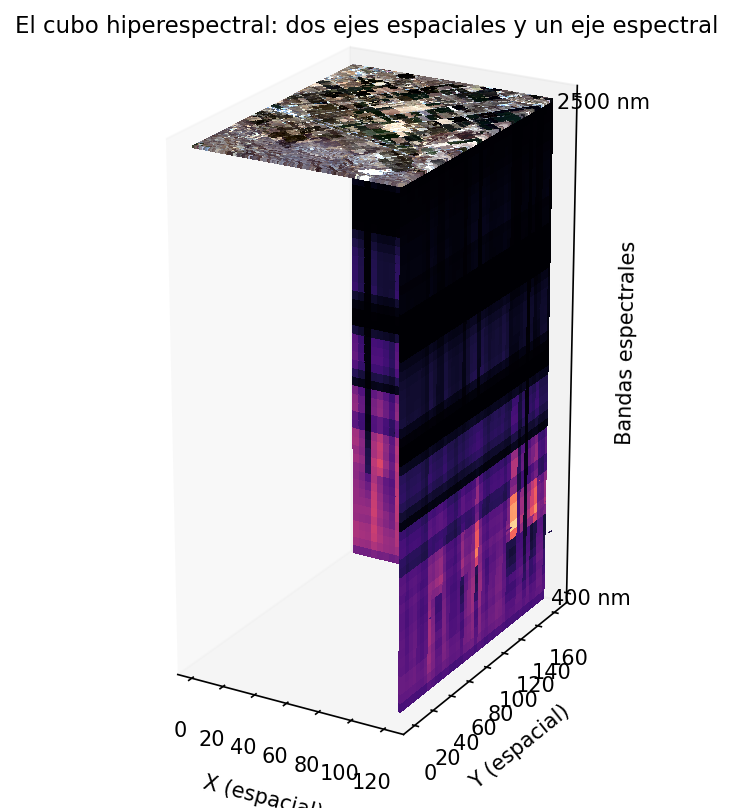
\includegraphics[width=0.55\linewidth]{hipercubo.png}
\nota{La cara superior corresponde a la escena y las caras laterales muestran la variación a lo largo de las bandas. Elaborada con datos del conjunto Santa Barbara \parencite{hasanlou2018hyperspectral}.}
\end{figure}

\begin{figure}[htbp]
\caption{Firmas espectrales de distintos puntos de la escena de prueba}
\label{fig:firmas}
\centering
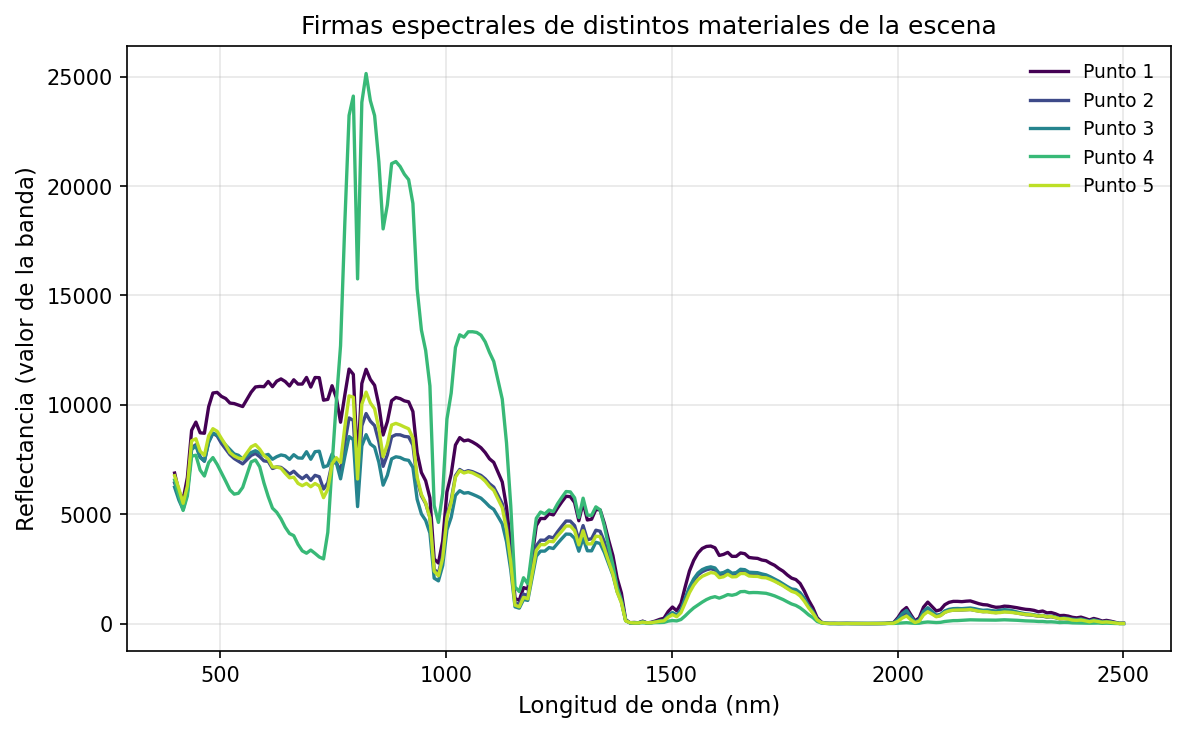
\includegraphics[width=0.8\linewidth]{firmas_espectrales.png}
\nota{Cada material describe una curva propia de reflectancia frente a la longitud de onda; el punto 4 sobre vegetación muestra un salto característico en el infrarrojo cercano. Elaborada con datos del conjunto Santa Barbara \parencite{hasanlou2018hyperspectral}.}
\end{figure}

\subsubsection{Detección de cambios bitemporales}

La detección de cambios consiste en comparar dos o más imágenes del mismo lugar capturadas en momentos distintos para identificar las regiones donde se produjo una modificación. En teledetección es una tarea central para el monitoreo del territorio, la evaluación de desastres y el seguimiento del uso del suelo. Actualmente existen técnicas basadas en aprendizaje profundo, que permiten aprender representaciones que capturan información semántica y dan mejores resultados frente a variaciones de iluminación y registro, en lugar de operar simplemente sobre diferencias de píxeles e índices espectrales, que se pueden ver afectados por múltiples factores \parencite{khelifi2020deep}. En este trabajo se usarán imágenes hiperespectrales para hacer detección de cambios bitemporal, por lo que se emplearán imágenes de la misma escena en tiempos diferentes, como se observa en la Figura~\ref{fig:bitemporal}. Se trata del par Santa Barbara, capturado en 2013 y 2014 por el sensor aerotransportado AVIRIS, que es uno de los conjuntos públicos que se usarán en este trabajo \parencite{hasanlou2018hyperspectral}.

\begin{figure}[htbp]
\caption{Par hiperespectral bitemporal Santa Barbara en dos fechas, mostrado como composición RGB}
\label{fig:bitemporal}
\centering
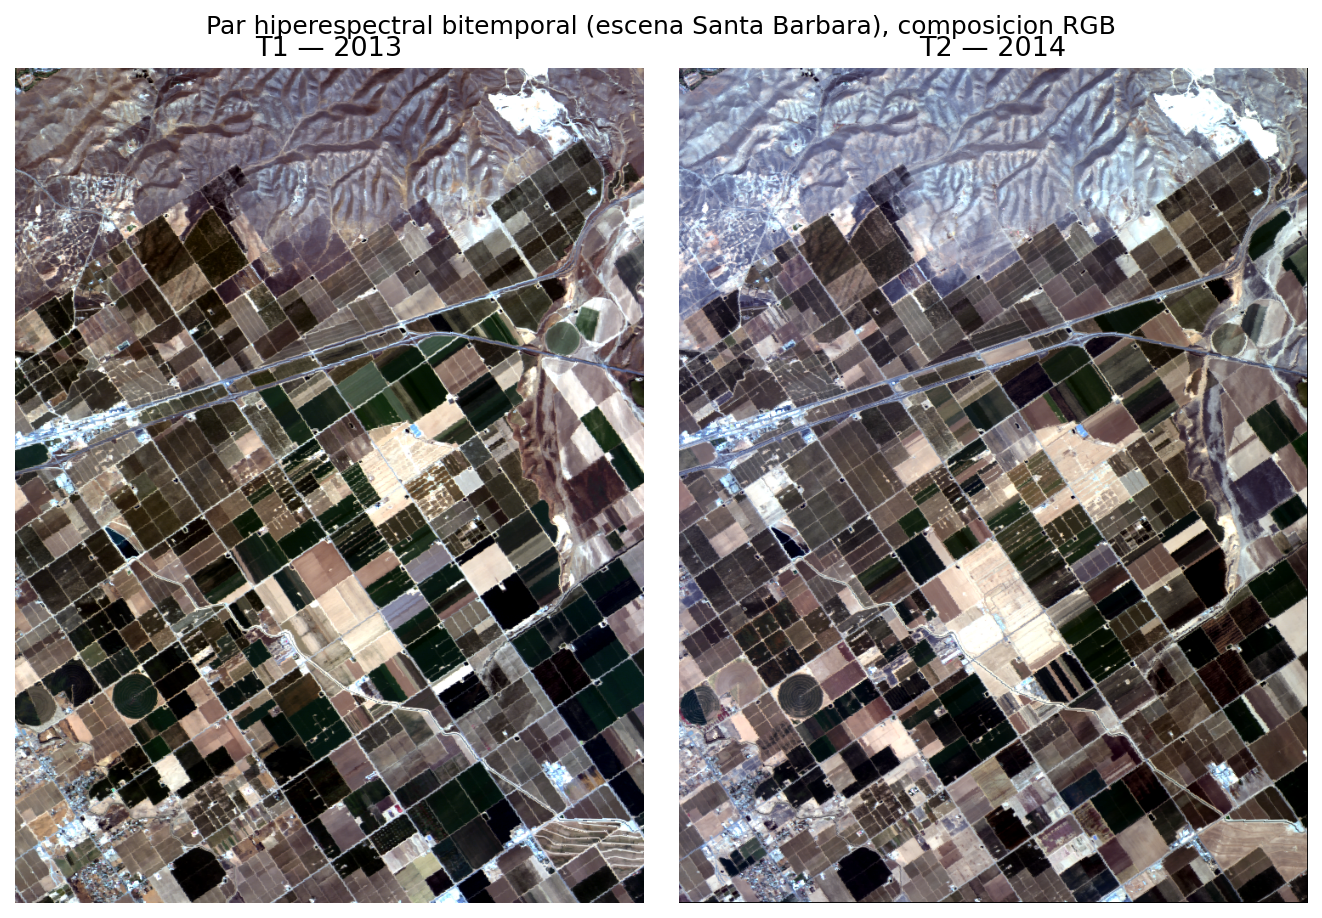
\includegraphics[width=\linewidth]{par_bitemporal.png}
\nota{La detección de cambios busca las regiones que difieren entre T1 y T2. Elaborada con datos del conjunto Santa Barbara \parencite{hasanlou2018hyperspectral}.}
\end{figure}

\subsubsection{Segmentación de imágenes}

La segmentación es la tarea de asignar a cada píxel de una imagen una etiqueta que lo agrupa en una región coherente, delimitando objetos o zonas con precisión a nivel de píxel. A diferencia de la clasificación, que asigna una única categoría a toda la imagen, la segmentación produce máscaras que separan cada elemento de la escena.

En cuanto a los modelos que existen, el enfoque tradicional se apoya en redes convolucionales de tipo codificador y decodificador, como U-Net, Mask R-CNN o DeepLab, que se entrenan de forma supervisada para un conjunto fijo de clases y un dominio concreto. El paradigma actual son los modelos fundacionales de segmentación promptable o guiado por indicaciones, cuyo referente es Segment Anything, entrenado sobre un conjunto de datos masivo y capaz de generar máscaras precisas a partir de indicaciones espaciales como puntos o recuadros, sin necesidad de reentrenarse para cada dominio \parencite{kirillov2023sam}. Modelos posteriores como SAM 2 extienden esta idea a video, pero comparten el mismo principio de segmentación guiada por indicaciones \parencite{ravi2024sam2}.

La aplicación de estos modelos a una imagen hiperespectral no es directa. Segment Anything está diseñado para imágenes naturales de tres canales y no puede recibir como entrada un cubo hiperespectral de cientos de bandas, por lo que se requiere proyectar toda esa información adicional a las tres bandas que puede procesar.

\subsubsection{Transformers y Vision Transformers}

El transformador, del inglés \textit{Transformer}, es una arquitectura de red neuronal basada por completo en el mecanismo de atención, que en lugar de procesar la información de forma local, como hace una convolución, pondera de manera explícita la relación entre todos los elementos de una secuencia y aprende cuáles son relevantes entre sí \parencite{vaswani2017attention}. El \textit{Vision Transformer} traslada esta idea a las imágenes: divide la imagen en parches de tamaño fijo, proyecta cada parche a un vector, los trata como una secuencia de fichas y aplica atención sobre ellos. Su ventaja frente a las redes convolucionales se manifiesta al preentrenarse con grandes volúmenes de datos, régimen en el que aprende representaciones muy transferibles, y por eso se ha convertido en la arquitectura base de los modelos fundacionales de visión \parencite{dosovitskiy2021vit}. La Figura~\ref{fig:vit} resume este flujo.

\begin{figure}[htbp]
\caption{Esquema del Vision Transformer}
\label{fig:vit}
\centering
\begin{singlespace}
\begin{tikzpicture}[font=\footnotesize, >=Stealth,
  caja/.style={draw, rounded corners=2pt, align=center, fill=azul2!35, inner sep=4pt, minimum height=1.5cm},
  sub/.style={draw, rounded corners=1pt, fill=white, minimum width=2.8cm, minimum height=0.5cm, align=center}]
\foreach \i in {0,1,2}{\foreach \j in {0,1,2}{\draw[fill=verde1!45] (\i*0.5,\j*0.5) rectangle ++(0.5,0.5);}}
\node[align=center] at (0.75,-0.5) {Imagen dividida\\en parches};
\node[caja] (proj) at (3.3,0.75) {Proyección\\lineal de\\cada parche};
\foreach \k in {0,...,4}{\draw[fill=lima1] (5.0,0.0+\k*0.32) rectangle ++(0.3,0.3);}
\node[align=center] at (5.15,-0.5) {Fichas con\\posición};
\node[sub] (ln1) at (8.0,1.65) {Normalización};
\node[sub] (att) at (8.0,1.05) {Atención multicabeza};
\node[sub] (ln2) at (8.0,0.45) {Normalización};
\node[sub] (mlp) at (8.0,-0.15) {Perceptrón multicapa};
\begin{scope}[on background layer]
\node[draw, rounded corners=3pt, fill=morado1!20, fit=(ln1)(mlp), inner sep=6pt] (enc) {};
\end{scope}
\node[below=2pt of enc] {Codificador Transformer, $L$ bloques};
\node[caja, fill=lima1!60] (out) at (11.6,0.75) {Vectores de\\características};
\draw[->] (1.6,0.75) -- (proj.west);
\draw[->] (proj.east) -- (4.9,0.75);
\draw[->] (5.4,0.75) -- (enc.west);
\draw[->] (enc.east) -- (out.west);
\end{tikzpicture}
\end{singlespace}
\nota{La imagen se divide en parches, cada parche se proyecta a una ficha con su posición y la secuencia de fichas pasa por $L$ bloques de atención que producen los vectores de características. Adaptado de \textcite{dosovitskiy2021vit}.}
\end{figure}

Formalmente, la atención de producto punto escalado calcula, a partir de las matrices de consultas $Q$, claves $K$ y valores $V$,
\begin{equation}
\operatorname{Attention}(Q,K,V)=\operatorname{softmax}\!\left(\frac{QK^{\top}}{\sqrt{d_k}}\right)V,
\end{equation}
donde $d_k$ es la dimensión de las claves y el factor $\sqrt{d_k}$ evita que el producto crezca demasiado y sature la función softmax. Cada elemento de la secuencia queda así representado como una combinación ponderada de los demás, con pesos que expresan su relevancia mutua \parencite{vaswani2017attention}.

\subsubsection{Modelos fundacionales}

Un modelo fundacional es un modelo de gran escala preentrenado sobre cantidades masivas de datos, diseñado para servir como base reutilizable en múltiples tareas posteriores sin necesidad de entrenarlo desde cero. Para imágenes hiperespectrales, HyperSIGMA es el primer modelo fundacional con más de mil millones de parámetros, preentrenado sobre un conjunto extenso de imágenes, capaz de extraer características espaciales y espectrales transferibles a tareas como clasificación, detección de cambios y segmentación \parencite{wang2024hypersigma}. Esto permite aprovechar su gran capacidad de generalización, así como la posibilidad de usar modelos ya entrenados con más datos de los que normalmente se tendrían disponibles; entrenar uno desde cero sería una tarea compleja y posiblemente daría resultados inferiores debido a las limitaciones de datos de entrenamiento y de equipo necesario.

En los últimos años, los modelos fundacionales se han convertido en una herramienta central de la investigación en visión por computadora y teledetección. Su capacidad de transferir el conocimiento adquirido en el preentrenamiento a tareas nuevas, con pocos o ningún ejemplo etiquetado, ha impulsado su adopción en problemas donde los datos anotados son escasos o costosos, como ocurre con las imágenes hiperespectrales. Esta tendencia se refleja en la aparición de modelos fundacionales propios del dominio \parencite{wang2024hypersigma}, en enfoques de clasificación sin entrenamiento específico \parencite{pang2025special} y en la detección de cambios semánticos apoyada en estos modelos \parencite{zhu2025semanticcd}.

\subsubsection{Arquitectura de HyperSIGMA: SpatViT y atención por muestreo disperso}

La extracción de características de este trabajo recaerá en SpatViT, la subred espacial de HyperSIGMA. Es un Vision Transformer que divide la imagen hiperespectral en parches no solapados y los procesa con atención; en la variante base que se buscará emplear, esta produce un mapa de características denso \parencite{wang2024hypersigma}.

El problema es que la autoatención completa tiene un costo cuadrático en el número de fichas, y las imágenes hiperespectrales presentan una fuerte redundancia espacial y espectral, por lo que atender de forma uniforme a todas las posiciones es ineficiente. SpatViT lo resuelve con la atención por muestreo disperso. En lugar de comparar cada consulta con todas las claves, cada consulta $\mathbf{q}$ predice $N_p$ desplazamientos de muestreo mediante una proyección lineal aprendida $W_p$, y las claves y los valores se muestrean únicamente en esas posiciones desplazadas mediante interpolación bilineal, formando los conjuntos reducidos $K'$ y $V'$. La atención se calcula entonces solo sobre ese conjunto disperso:
\begin{equation}
\operatorname{SSA}(Q,K',V')=\operatorname{softmax}\!\left(\frac{Q\,K'^{\top}}{\sqrt{D'}}\right)V',
\end{equation}
donde $D'$ es la dimensión de las claves. Así, cada consulta aprende qué regiones son relevantes en vez de recorrerlas todas, lo que captura contexto diverso de largo alcance con un costo mucho menor que la autoatención completa \parencite{wang2024hypersigma}.

\subsubsection{Aprendizaje zero-shot}

El aprendizaje zero-shot se refiere a la capacidad de un modelo para resolver una tarea o reconocer categorías que no aparecieron durante su entrenamiento, apoyándose en el conocimiento general adquirido en el preentrenamiento. Modelos como CLIP usan esta técnica para clasificar imágenes en categorías descritas únicamente mediante texto, sin haber visto ejemplos etiquetados de esas categorías \parencite{radford2021clip}. En el ámbito hiperespectral, trabajos recientes llevan esta idea a la clasificación de coberturas del suelo, o \textit{land covers}, sin entrenamiento específico \parencite{pang2025special}. El sistema propuesto es zero-shot en tanto no requiere entrenar sobre pares de imágenes hiperespectrales etiquetados para detectar y nombrar los cambios. Esto está alineado con el uso de modelos fundacionales, ya que el enfoque permite aprovechar todas sus ventajas sin tener que entrenar necesariamente un modelo propio.

\subsubsection{Vocabulario abierto}

El enfoque de vocabulario abierto permite etiquetar regiones de una imagen con cualquier concepto expresable en lenguaje natural, en lugar de restringirse a un conjunto cerrado y predefinido de clases. Un clasificador clásico se entrena sobre un número fijo de categorías, por ejemplo agua, vegetación o edificación, y solo puede responder con una de esas etiquetas aprendidas. Si aparece un concepto nuevo que no estaba en ese conjunto, el modelo no puede nombrarlo, y para agregarlo hay que anotar datos nuevos y volver a entrenar la red por completo, por lo cual no es muy práctico.

El vocabulario abierto funciona de otra forma y soluciona el problema. En lugar de una capa final con un número fijo de salidas, se emplean modelos que proyectan imágenes y texto a un mismo espacio de representación, de tal modo que la etiqueta se decide comparando la región con la descripción textual de cada categoría candidata \parencite{radford2021clip}. Las categorías ya no son fijas en la red, sino que se entregan como texto en el momento de la consulta, y pueden cambiarse o ampliarse sin reentrenar nada \parencite{kombol2025trainingfree}.

El vocabulario tradicional funciona como una especie de formulario en donde solo se puede elegir entre opciones predeterminadas, mientras que el vocabulario abierto funciona más como un prompt, en donde se escribe con lenguaje natural y el modelo decide cuál opción encaja mejor con la imagen.

\subsubsection{Modelos de visión-lenguaje y descripción de imágenes}

Los modelos de visión-lenguaje aprenden una representación conjunta de imágenes y texto a partir de grandes colecciones de pares imagen y descripción, con el fin de resolver tareas visuales guiadas por lenguaje sin entrenar un modelo distinto para cada una \parencite{zhang2024vlm}. CLIP es el exponente que se buscará emplear en este trabajo: entrena dos codificadores, uno visual y uno textual, para proyectar ambas modalidades a un espacio común donde la correspondencia se mide por similitud, lo que habilita la clasificación por texto libre y el etiquetado de vocabulario abierto \parencite{radford2021clip}. La Figura~\ref{fig:clip} ilustra cómo se aplicará este principio para etiquetar una región de cambio.

\begin{figure}[htbp]
\caption{Etiquetado de vocabulario abierto con CLIP}
\label{fig:clip}
\centering
\begin{singlespace}
\begin{tikzpicture}[font=\footnotesize, >=Stealth,
  caja/.style={draw, rounded corners=2pt, align=center, inner sep=4pt},
  vec/.style={draw, minimum width=1.0cm, minimum height=0.6cm}]
\node[caja, fill=lima1!60, text width=3.6cm, font=\scriptsize] (txt) at (0,2.6) {``imagen de deforestación''\\``imagen de inundación''\\``imagen de zona urbana''};
\node[caja, fill=azul2!40] (tenc) at (3.7,2.6) {Codificador\\de texto};
\node[caja, fill=verde1!40, minimum width=1.6cm, minimum height=1.2cm] (img) at (0,0) {Región\\de cambio};
\node[caja, fill=azul2!40] (ienc) at (3.7,0) {Codificador\\de imagen};
\foreach \j/\l in {0/T_1,1/T_2,2/T_3}{\node[vec, fill=lima1] (t\j) at (6.6+\j*1.1,2.6) {$\l$};}
\node[vec, fill=verde1!50] (i0) at (5.4,0) {$I$};
\node[vec, fill=morado1!35] (s0) at (6.6,0) {$\scriptstyle I\cdot T_1$};
\node[vec, fill=white] (s1) at (7.7,0) {$\scriptstyle I\cdot T_2$};
\node[vec, fill=white] (s2) at (8.8,0) {$\scriptstyle I\cdot T_3$};
\draw[->] (txt) -- (tenc);
\draw[->] (tenc) -- (t0);
\draw[->] (img) -- (ienc);
\draw[->] (ienc) -- (i0);
\foreach \j in {0,1,2}{\draw[->, dashed, gray] (t\j.south) -- (s\j.north);}
\node[align=center, font=\scriptsize] at (7.7,-0.85) {Similitud coseno en el espacio común;\\la región recibe la etiqueta de mayor similitud};
\end{tikzpicture}
\end{singlespace}
\nota{La región y cada descripción candidata se proyectan a un espacio común y la región se etiqueta con la descripción más similar. El vocabulario puede cambiarse sin reentrenar. Adaptado de \textcite{radford2021clip}.}
\end{figure}

La descripción de imágenes, también llamada generación de subtítulos, va un paso más allá de la clasificación: en vez de asignar una etiqueta, genera una frase en lenguaje natural que resume el contenido visual. Los primeros modelos neuronales de esta tarea se dividen en dos fases, un codificador convolucional que condensa la imagen en un vector y un decodificador recurrente que, a partir de ese vector, produce la frase palabra por palabra; sus autores lo describen como un modelo que ``se puede usar para generar frases naturales que describen una imagen'' \parencite{vinyals2015show}. Hoy la línea la dominan los modelos de visión-lenguaje preentrenados a gran escala, como BLIP, que reúnen en una sola arquitectura la comprensión de la imagen y la generación del texto que la describe \parencite{li2022blip}.

En teledetección, la descripción de imágenes se apoya en conjuntos de datos propios. RSICD, por ejemplo, reúne cerca de once mil imágenes de teledetección con varias descripciones cada una, y permite entrenar y evaluar modelos adaptados a las escenas aéreas y satelitales \parencite{lu2017rsicd}. Esos avances se dieron sobre imágenes ópticas de tres canales y no hiperespectrales. La extensión al dominio hiperespectral llegó con HyperCap, el primer punto de referencia para describir coberturas de terreno a partir de imágenes hiperespectrales, que hace posible aplicar modelos de visión-lenguaje sobre el cubo espectral completo \parencite{das2025hypercap}.

\subsubsection{Representaciones vectoriales y similitud coseno}

El aprendizaje profundo parte de que el desempeño en una tarea depende sobre todo de la calidad de la representación de los datos \parencite{bengio2013representation}. Un modelo profundo transforma cada imagen o región en un vector de características o \textit{embedding} $\mathbf{v}\in\mathbb{R}^{d}$, con $d$ del orden de cientos, en un espacio donde la proximidad entre vectores corresponde a similitud semántica.

La comparación entre dos \textit{embeddings} $\mathbf{u}$ y $\mathbf{v}$ usa la similitud coseno:
\begin{equation}
\operatorname{sim}(\mathbf{u},\mathbf{v})=\frac{\mathbf{u}\cdot\mathbf{v}}{\lVert\mathbf{u}\rVert\,\lVert\mathbf{v}\rVert}=\frac{\sum_{i=1}^{d}u_i v_i}{\sqrt{\sum_{i=1}^{d}u_i^{2}}\,\sqrt{\sum_{i=1}^{d}v_i^{2}}}\in[-1,1].
\end{equation}
La normalización por las magnitudes $\lVert\mathbf{u}\rVert$ y $\lVert\mathbf{v}\rVert$ elimina la escala y conserva solo la orientación, por lo que la medida es insensible a diferencias de brillo o ganancia entre las dos capturas.

En detección de cambios, esta similitud permite comparar las representaciones de dos imágenes de una misma escena adquiridas en momentos distintos. Si $\mathbf{e}_1(p)$ y $\mathbf{e}_2(p)$ son los \textit{embeddings} asociados a una misma posición $p$ en la imagen inicial y en la final, una medida de cambio puede definirse como
\begin{equation}
C(p)=1-\operatorname{sim}\!\big(\mathbf{e}_1(p),\mathbf{e}_2(p)\big),
\end{equation}
de modo que un valor alto indica cambio y uno bajo, permanencia. De forma análoga, la similitud coseno permite comparar \textit{embeddings} de distinta modalidad, como el de una región de imagen y el de una descripción textual, siempre que ambos estén proyectados en un espacio común. La Figura~\ref{fig:mapacambio} muestra un mapa de cambio de este tipo calculado sobre el par Santa Barbara con un prototipo preliminar del sistema.

\begin{figure}[htbp]
\caption{Mapa de cambio $C(p)$ obtenido con similitud coseno entre las representaciones de HyperSIGMA del par Santa Barbara}
\label{fig:mapacambio}
\centering
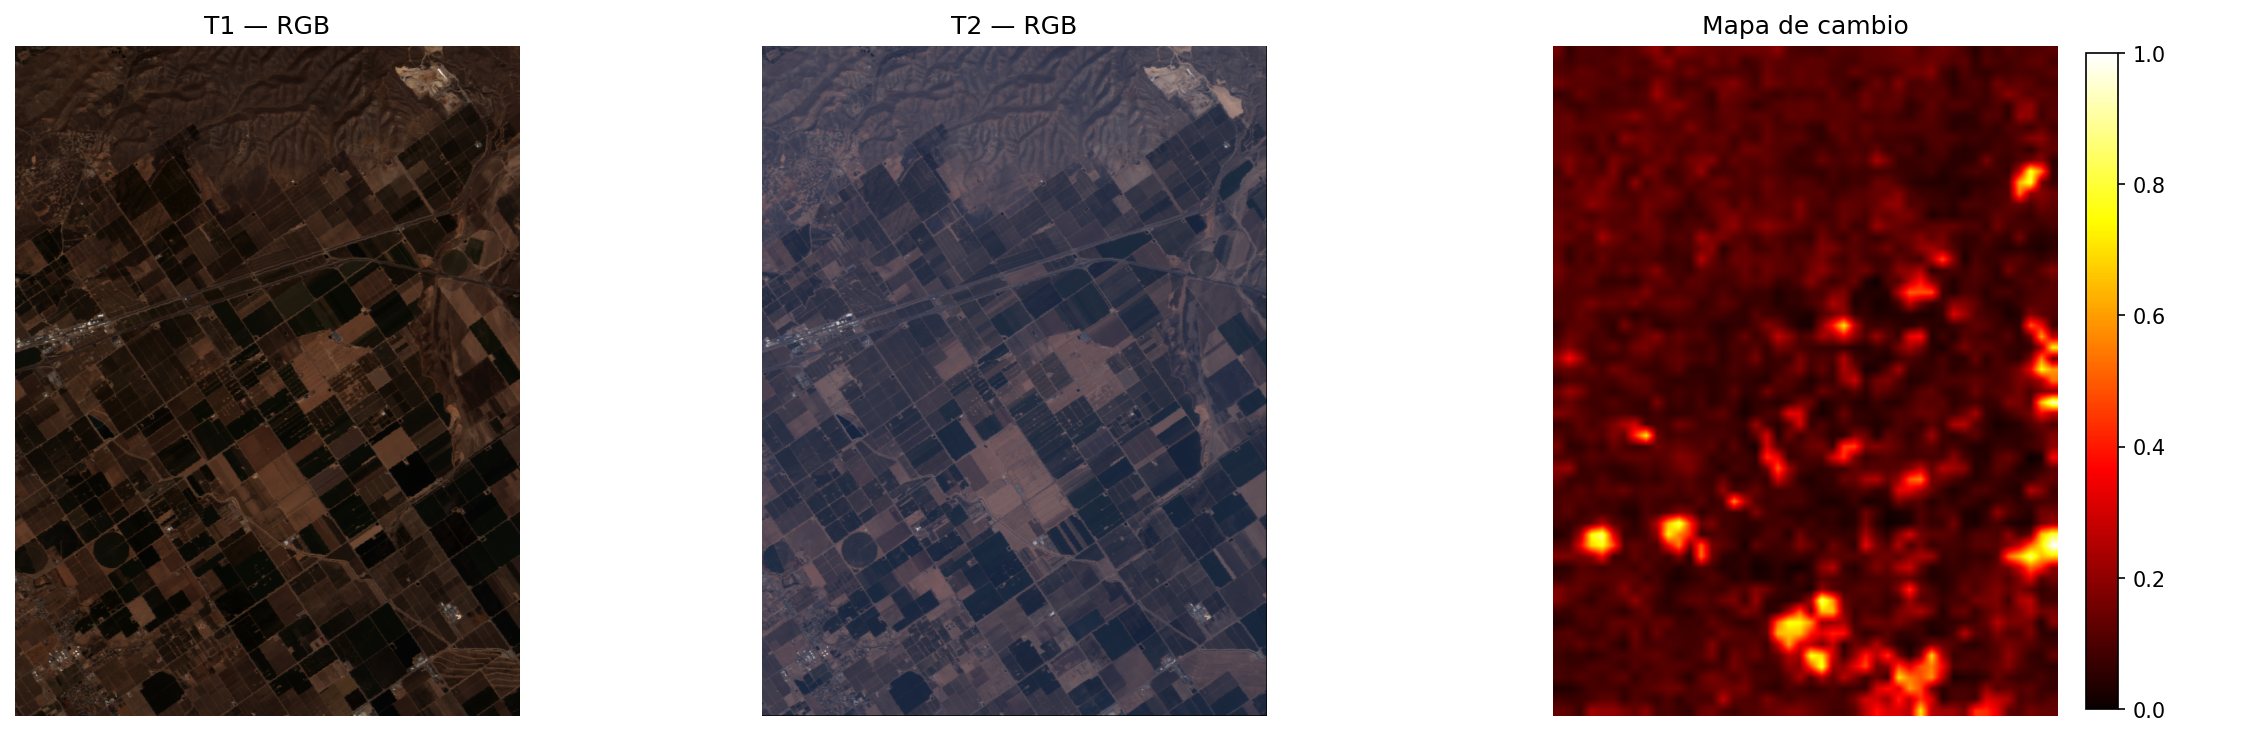
\includegraphics[width=\linewidth]{mapa_cambio.png}
\nota{Los valores cercanos a uno, en tonos claros, señalan las zonas donde la representación varió entre T1 y T2. Elaborada con datos del conjunto Santa Barbara \parencite{hasanlou2018hyperspectral}.}
\end{figure}

\subsubsection{Métricas de evaluación}

La evaluación de la detección de cambios se plantea como una comparación píxel a píxel entre el resultado del sistema y un mapa de referencia anotado, conocido como \textit{ground truth}, de la que surgen cuatro conteos: verdaderos positivos $VP$ cuando se detecta un cambio real, verdaderos negativos $VN$ cuando se identifica correctamente una zona sin cambio, falsos positivos $FP$ cuando se señala un cambio inexistente y falsos negativos $FN$ cuando se pasa por alto un cambio real. Estos conteos se organizan en la matriz de confusión de la Figura~\ref{fig:confusion}, y sobre ellos se definen las métricas de desempeño.

\begin{figure}[htbp]
\caption{Matriz de confusión de la detección de cambios}
\label{fig:confusion}
\centering
\begin{singlespace}
\begin{tikzpicture}[font=\footnotesize,
  cel/.style={draw, minimum width=3.4cm, minimum height=1.4cm, align=center}]
\node[cel, fill=lima1] at (0,0) {$VP$\\cambio real\\detectado};
\node[cel, fill=morado1!25] at (3.4,0) {$FP$\\cambio señalado\\inexistente};
\node[cel, fill=morado1!25] at (0,-1.4) {$FN$\\cambio real\\no detectado};
\node[cel, fill=lima1] at (3.4,-1.4) {$VN$\\sin cambio\\identificado};
\node at (0,1.0) {\textbf{Cambio}};
\node at (3.4,1.0) {\textbf{Sin cambio}};
\node at (1.7,1.5) {\textbf{\textit{Ground truth}}};
\node[anchor=east] at (-1.85,0) {\textbf{Cambio}};
\node[anchor=east] at (-1.85,-1.4) {\textbf{Sin cambio}};
\node[rotate=90] at (-4.0,-0.7) {\textbf{Predicción}};
\end{tikzpicture}
\end{singlespace}
\nota{Las celdas de la diagonal son aciertos y las demás son errores del sistema.}
\end{figure}

La precisión $P$ mide qué proporción de los cambios detectados son correctos y penaliza los falsos positivos, mientras que la exhaustividad $R$ mide qué proporción de los cambios reales se detectaron y penaliza los falsos negativos:
\begin{equation}
P=\frac{VP}{VP+FP},\qquad R=\frac{VP}{VP+FN}.
\end{equation}
Como suele existir una tensión entre ambas, el puntaje F1 las combina en un único valor mediante su media armónica, que solo es alta cuando las dos lo son:
\begin{equation}
F_1=\frac{2\,P\,R}{P+R}=\frac{2\,VP}{2\,VP+FP+FN}.
\end{equation}
La intersección sobre unión evalúa el solapamiento espacial entre la región detectada y la real, dividiendo el área común entre el área total que cubren juntas:
\begin{equation}
\mathrm{IoU}=\frac{VP}{VP+FP+FN}.
\end{equation}
Estas métricas son el estándar en la revisión de métodos de detección de cambios basados en aprendizaje profundo \parencite{khelifi2020deep}. En este trabajo serán la base de la validación cuantitativa del sistema: la máscara de cambio producida por el pipeline se contrastará con el \textit{ground truth} de los conjuntos hiperespectrales bitemporales Santa Barbara, Bay Area y River, y los valores de precisión, exhaustividad y puntaje F1 permitirán situar el desempeño frente a métodos existentes.

\subsubsection{Modelos y datos empleados en el sistema propuesto}

Las tres piezas centrales del pipeline comparten el mismo esqueleto arquitectónico, el Vision Transformer. En la extracción de características, HyperSIGMA procesará cada imagen con un codificador de tipo Vision Transformer espacial, en su variante base, que divide el cubo en parches y produce mapas de características densos a partir de los cuales se calculará el mapa de cambio \parencite{wang2024hypersigma}. En la segmentación, Segment Anything delimitará las regiones con un codificador de imagen Vision Transformer \parencite{kirillov2023sam}. Y en el etiquetado, CLIP asignará las etiquetas de vocabulario abierto mediante un codificador visual Vision Transformer alineado con el texto \parencite{radford2021clip}. Así, el mismo principio de atención sobre parches recorre la detección de características, la segmentación y el etiquetado, lo que da coherencia arquitectónica a todo el sistema.

A continuación se reúnen las tecnologías que se estudiarán y revisarán para el desarrollo de este proyecto:
\begin{itemize}[leftmargin=1.27cm]
  \item \textbf{HyperSIGMA} --- modelo fundacional hiperespectral basado en Vision Transformer, escalable a más de mil millones de parámetros y preentrenado sobre un conjunto masivo de imágenes hiperespectrales. Extraerá las representaciones profundas de cada imagen, sobre las que se calculará el mapa de cambio \parencite{wang2024hypersigma}.
  \item \textbf{Segment Anything} --- modelo fundacional de segmentación promptable con codificador Vision Transformer de gran tamaño. Convertirá las regiones de cambio en máscaras precisas a nivel de píxel a partir de indicaciones espaciales \parencite{kirillov2023sam}.
  \item \textbf{CLIP} --- modelo de visión-lenguaje que alinea imagen y texto en un espacio común. Asignará a cada región una etiqueta de vocabulario abierto por similitud entre la imagen y las descripciones textuales candidatas \parencite{radford2021clip}.
  \item \textbf{BLIP} --- modelo de visión-lenguaje que unifica comprensión y generación. Generaría la descripción en lenguaje natural de cada región, una vez adaptado a datos hiperespectrales \parencite{li2022blip}.
  \item \textbf{HyperCap} --- primer conjunto de datos y punto de referencia para la descripción de imágenes hiperespectrales, con anotaciones textuales a nivel de píxel. Servirá de base de entrenamiento y evaluación del módulo de descripción \parencite{das2025hypercap}.
\end{itemize}

Para el desarrollo y la evaluación de la detección de cambios se emplearán tres conjuntos públicos de pares hiperespectrales bitemporales, todos con \textit{ground truth} que indica qué píxeles cambiaron entre las dos fechas:
\begin{itemize}[leftmargin=1.27cm]
  \item \textbf{Santa Barbara} --- par capturado en 2013 y 2014 por el sensor aerotransportado AVIRIS, de 984 por 740 píxeles y 224 bandas, sobre una zona agrícola y urbana de California. Será el par principal de desarrollo del sistema \parencite{hasanlou2018hyperspectral}.
  \item \textbf{Bay Area} --- par capturado en 2013 y 2015 por el mismo sensor AVIRIS, de 600 por 500 píxeles y 224 bandas, publicado junto con Santa Barbara \parencite{hasanlou2018hyperspectral}.
  \item \textbf{River} --- par capturado por el sensor Hyperion del satélite EO-1, publicado por los autores de GETNET como conjunto de referencia para comparar métodos de detección de cambios hiperespectral \parencite{wang2019getnet}. Al provenir de Hyperion, coincide con el espacio espectral de referencia del modelo de extracción de características.
\end{itemize}

\subsection{Estado del Arte}

El estado del arte se presenta siguiendo la metodología propuesta. Para cada etapa se realizó una revisión sobre cómo se resuelve el problema actualmente, qué alternativas existen y finalmente se justifican las herramientas elegidas para llevar a cabo este proyecto. La Figura~\ref{fig:lineatiempo} ubica en el tiempo los trabajos que se revisan en esta sección.

\begin{figure}[htbp]
\caption{Línea de tiempo de los trabajos que fundamentan este proyecto, desde la espectrometría de imagen hasta los modelos fundacionales hiperespectrales y de visión-lenguaje}
\label{fig:lineatiempo}
\centering
\begin{singlespace}
\resizebox{\linewidth}{!}{%
\begin{tikzpicture}[font=\scriptsize]
\draw[very thick, verde1, -{Stealth}] (-0.6,0) -- (14.9,0);
\foreach \a/\t [count=\k from 0] in {
  1985/{Espectrometría\\de imagen},
  2009/{Aprendizaje\\zero-shot},
  2015/{U-Net y\\Show and Tell},
  2017/{Transformer y\\Mask R-CNN},
  2018/{Conjuntos Santa\\Barbara y Bay Area},
  2019/{GETNET y\\conjunto River},
  2021/{Vision Transformer\\y CLIP},
  2022/{BLIP},
  2023/{Segment\\Anything},
  2024/{HyperSIGMA\\y SAM 2},
  2025/{Semantic-CD,\\SPECIAL y HyperCap},
  2026/{Este trabajo:\\OVCD hiperespectral}}{
  \pgfmathsetmacro{\x}{\k*1.28}
  \fill[morado1] (\x,0) circle (2.2pt);
  \ifodd\k
    \draw[gray] (\x,0) -- (\x,-0.7);
    \node[below, align=center, text width=2.2cm] at (\x,-0.7) {\textbf{\a}\\\t};
  \else
    \draw[gray] (\x,0) -- (\x,0.7);
    \node[above, align=center, text width=2.2cm] at (\x,0.7) {\textbf{\a}\\\t};
  \fi
}
\end{tikzpicture}}
\end{singlespace}
\nota{Basada en \textcite{goetz1985imaging}, \textcite{palatucci2009zeroshot}, \textcite{ronneberger2015unet}, \textcite{vinyals2015show}, \textcite{vaswani2017attention}, \textcite{he2017maskrcnn}, \textcite{hasanlou2018hyperspectral}, \textcite{wang2019getnet}, \textcite{dosovitskiy2021vit}, \textcite{radford2021clip}, \textcite{li2022blip}, \textcite{kirillov2023sam}, \textcite{wang2024hypersigma}, \textcite{ravi2024sam2}, \textcite{zhu2025semanticcd}, \textcite{pang2025special} y \textcite{das2025hypercap}.}
\end{figure}

\subsubsection{Imágenes hiperespectrales y su adquisición}

La imagen hiperespectral nace de la espectrometría de imagen, formulada por Goetz en 1985 como la adquisición simultánea de imágenes en muchas bandas espectrales contiguas para obtener, en cada píxel, un espectro completo con el que identificar los materiales de la superficie terrestre \parencite{goetz1985imaging}. La tecnología ha evolucionado en gran medida desde los primeros sensores aerotransportados, como AVIRIS del Jet Propulsion Laboratory de la NASA, hacia sensores satelitales como Hyperion del satélite EO-1, que amplían el rango de cobertura y permiten disponer de más datos con cientos de bandas \parencite{bhargava2024hyperspectral}. Además de los sensores de barrido, existen también cámaras instantáneas que capturan todo el cubo a la vez, pero pierden resolución frente a las otras alternativas; siempre hay una relación de compromiso entre resolución espacial, resolución espectral y relación señal a ruido, y hay que decidir qué característica se prioriza frente a las demás. En este trabajo los datos entrarán como pares bitemporales en formatos ENVI, MATLAB o GeoTIFF, concretamente los conjuntos Santa Barbara y Bay Area, del sensor AVIRIS \parencite{hasanlou2018hyperspectral}, y River, del sensor Hyperion \parencite{wang2019getnet}, y se reinterpolarán a un espacio espectral de referencia, el del sensor Hyperion, que es el mismo sobre el que fue preentrenado el modelo fundacional de extracción de características.

\subsubsection{Extracción de características: transformers y modelos fundacionales hiperespectrales}

Para obtener la representación de la imagen hiperespectral hay dos formas principales. La tradicional es calcularla a mano mediante índices espectrales, fórmulas que combinan bandas concretas para resaltar un material; el problema es que para saber qué fórmula usar y de qué modo, se necesita saber de antemano qué se quiere resaltar. La alternativa moderna, que adoptará este trabajo, es aprenderla con un modelo fundacional. HyperSIGMA representa la imagen dividiendo el cubo en parches y procesándolos con un Vision Transformer espacial que, mediante su atención por muestreo disperso, produce un mapa denso de vectores de características, uno por posición, que codifican de forma conjunta la información espacial y espectral de la escena. Es el primer modelo fundacional hiperespectral con más de mil millones de parámetros, desarrollado por Wang, de la Universidad de Wuhan, y preentrenado sobre el conjunto HyperGlobal-450K con cerca de 450.000 imágenes \parencite{wang2024hypersigma}. La elección se justifica inicialmente porque estas representaciones son de mejor calidad que las de un índice manual y, al haberse aprendido sobre datos hiperespectrales, resultan transferibles a tareas nuevas sin necesidad de reentrenar. El código es público en el repositorio oficial del grupo WHU-Sigma \parencite{whu2024hypersigma_repo}.

\subsubsection{Detección de cambios y el emparejamiento en el espacio latente}

Las técnicas se agrupan en cuatro grupos. Las de álgebra de imágenes trabajan directamente sobre los valores de los píxeles, como la diferencia, el cociente o el análisis de vectores de cambio. Las de transformación proyectan los datos a otro espacio antes de compararlos, por ejemplo con PCA. Las de comparación post-clasificación clasifican cada imagen por separado y luego contrastan las clases. Y, de forma dominante hoy, las de aprendizaje profundo aprenden a detectar el cambio con redes siamesas y de atención \parencite{khelifi2020deep}. La Figura~\ref{fig:taxonomia} resume esta clasificación y ubica en ella el enfoque de este trabajo. La detección de cambios opera sobre imágenes multiespectrales, de radar de apertura sintética y, cada vez más, hiperespectrales, donde la alta resolución espectral permite detectar cambios pequeños; un ejemplo es GETNET, una red convolucional 2D de extremo a extremo que clasifica cada píxel como cambiado o no cambiado usando información de abundancia subpíxel obtenida por desmezclado espectral, y cuyos autores publicaron el conjunto de datos River \parencite{wang2019getnet}.

\begin{figure}[htbp]
\caption{Clasificación de las técnicas de detección de cambios y ubicación del enfoque propuesto dentro del aprendizaje profundo}
\label{fig:taxonomia}
\centering
\begin{singlespace}
\begin{tikzpicture}[font=\footnotesize, >=Stealth,
  raiz/.style={draw, rounded corners=3pt, fill=morado1!30, align=center, inner sep=5pt},
  rama/.style={draw, rounded corners=2pt, fill=azul2!35, align=center, text width=3cm, minimum height=1.1cm},
  hoja/.style={align=center, text width=3.2cm, font=\scriptsize}]
\node[raiz] (r) at (0,0) {Técnicas de detección de cambios};
\foreach \n/\x/\t/\d in {
  a/-5.4/{Álgebra de\\imágenes}/{Diferencia, cociente y\\vectores de cambio},
  b/-1.8/{Transformación}/{Proyección a otro\\espacio, como PCA},
  c/1.8/{Comparación\\post-clasificación}/{Clasificar cada fecha\\y contrastar clases},
  d/5.4/{Aprendizaje\\profundo}/{Redes siamesas\\y de atención}}{
  \node[rama] (\n) at (\x,-1.7) {\t};
  \node[hoja, below=3pt of \n] (h\n) {\d};
  \draw[->] (r.south) -- ++(0,-0.45) -| (\n.north);
}
\node[draw, dashed, rounded corners=2pt, fill=lima1!60, align=center, text width=3.6cm, font=\scriptsize] (e) at (5.4,-4.1) {Este trabajo: comparación zero-shot en el espacio latente de un modelo fundacional};
\draw[->, dashed] (hd.south) -- (e.north);
\end{tikzpicture}
\end{singlespace}
\nota{Adaptado de \textcite{khelifi2020deep}.}
\end{figure}

La mayoría de estos métodos requiere entrenar con pares etiquetados, escasos en el dominio hiperespectral. La alternativa que se buscará adoptar en este trabajo es saltar el entrenamiento: se compararán las representaciones que HyperSIGMA extraiga de las dos capturas mediante la similitud coseno, emparejando vectores en un espacio latente común; cuando la similitud entre las representaciones inicial y final sea baja, se considerará que hay cambio. Esta es la misma métrica que usan modelos como CLIP \parencite{radford2021clip}. La técnica se justifica por ser un enfoque zero-shot, que no depende de datos etiquetados de cambio y aprovecha directamente la calidad de las representaciones del modelo fundacional.

\subsubsection{Segmentación}

El estado del arte pasa de las redes convolucionales de codificador y decodificador entrenadas para un conjunto fijo de clases, como U-Net \parencite{ronneberger2015unet}, Mask R-CNN \parencite{he2017maskrcnn} y la familia DeepLab, a los modelos promptable. Segment Anything, desarrollado por Meta AI en 2023, se entrenó sobre el conjunto SA-1B, con once millones de imágenes y mil millones de máscaras \parencite{kirillov2023sam}; el modelo y sus pesos están disponibles en el sitio oficial \parencite{meta2023sam_repo}. Las alternativas entrenadas por clase exigirían anotar datos de las coberturas de interés, lo que no aborda la característica de vocabulario abierto del problema. Por esta razón se propone usar Segment Anything, porque produce máscaras precisas sin depender de clases predefinidas ni de reentrenamiento, y se integra de forma natural recibiendo como indicaciones los puntos y recuadros derivados del mapa de cambio, sobre una composición RGB del cubo hiperespectral.

\subsubsection{Etiquetado de vocabulario abierto}

El referente es CLIP, desarrollado por OpenAI en 2021 y entrenado por contraste sobre cerca de cuatrocientos millones de pares imagen-texto \parencite{radford2021clip}; su implementación oficial es pública \parencite{openai2021clip_repo}. En teledetección esta idea ya se traslada a la segmentación y la detección de cambios de vocabulario abierto \parencite{kombol2025trainingfree,zhu2025semanticcd}, y en el dominio hiperespectral a la clasificación zero-shot \parencite{pang2025special}. Este trabajo buscará usar CLIP porque convierte el etiquetado en una comparación por similitud contra un vocabulario de texto libre, editable sin reentrenar, que es la esencia del objetivo de vocabulario abierto; en el pipeline se asignará a cada máscara la etiqueta más afín de ese vocabulario.

\subsubsection{Descripción en lenguaje natural}

BLIP fue desarrollado por Salesforce Research en 2022 y su código es público \parencite{salesforce2022blip_repo}. La alternativa de aplicar un modelo de descripción de imágenes naturales ignora la información espectral del cubo. Por eso este trabajo, en su etapa de descripción, buscará adaptar un modelo de tipo BLIP \parencite{li2022blip} cuyo codificador visual se sustituirá por uno que reciba directamente el cubo hiperespectral, y que se entrenará sobre HyperCap \parencite{das2025hypercap}. Se justifica porque generaría una caracterización más rica que una sola etiqueta y aprovecharía la dimensión espectral completa.

\subsubsection{Aprendizaje zero-shot}

El término aparece con Palatucci en 2009, que predice clases nunca vistas mediante códigos de salida semánticos \parencite{palatucci2009zeroshot}, en paralelo con los enfoques basados en atributos de Lampert, que transfieren descripciones entre clases \parencite{lampert2009attribute}. Con el tiempo empiezan a surgir los modelos preentrenados a gran escala, como CLIP \parencite{radford2021clip}, y el zero-shot se consolida como una técnica ampliamente utilizada. Su validez reside en que un modelo fundacional, tras preentrenarse sobre volúmenes masivos de datos, captura conocimiento general y transferible, que permite generalizar a categorías nuevas siempre que se expresen en un espacio semántico común, por ejemplo el del lenguaje \parencite{wang2024hypersigma,radford2021clip}.

Las alternativas son el aprendizaje supervisado, que exige un conjunto etiquetado para cada tarea y clase; el ajuste fino de un modelo preentrenado, que necesita algunos ejemplos anotados; y el aprendizaje con pocos ejemplos, o few-shot. Todas requieren datos etiquetados del problema concreto. Este trabajo adoptará el enfoque zero-shot porque los pares hiperespectrales bitemporales con \textit{ground truth} son escasos y difíciles de anotar, ya que el proceso sería manual, y porque el objetivo mismo, detectar y nombrar cambios con vocabulario libre, es incompatible con un conjunto cerrado de clases.

\subsubsection{Vacío de investigación}

El estado del arte muestra que cada pieza está resuelta por separado: hay modelos fundacionales hiperespectrales \parencite{wang2024hypersigma}, segmentación promptable \parencite{kirillov2023sam}, etiquetado de vocabulario abierto \parencite{radford2021clip} y descripción hiperespectral \parencite{das2025hypercap}. El vocabulario abierto y el zero-shot están consolidados en imágenes RGB y empiezan a aparecer en teledetección \parencite{zhu2025semanticcd,kombol2025trainingfree}. Sin embargo, ninguna propuesta los integra para detectar y describir cambios, con vocabulario libre y sin entrenamiento, sobre imágenes hiperespectrales bitemporales. La Tabla~\ref{tab:vacio} contrasta los trabajos más cercanos con las características que exige el problema. Ese vacío es el que aborda este trabajo.

\begin{table}[htbp]
\caption{Comparación de los trabajos relacionados frente a las características del problema}
\label{tab:vacio}
\centering
\begin{singlespace}
\footnotesize
\begin{tabular}{lccccc}
\toprule
\textbf{Trabajo} & \makecell{\textbf{Imágenes}\\\textbf{hiperespectrales}} & \makecell{\textbf{Detección}\\\textbf{de cambios}} & \makecell{\textbf{Vocabulario}\\\textbf{abierto}} & \makecell{\textbf{Sin pares de}\\\textbf{cambio etiquetados}} & \makecell{\textbf{Descripción}\\\textbf{textual}} \\
\midrule
GETNET \parencite{wang2019getnet} & $\checkmark$ & $\checkmark$ & $\times$ & $\times$ & $\times$ \\
HyperSIGMA \parencite{wang2024hypersigma} & $\checkmark$ & $\checkmark$ & $\times$ & $\times$ & $\times$ \\
Semantic-CD \parencite{zhu2025semanticcd} & $\times$ & $\checkmark$ & $\checkmark$ & $\times$ & $\times$ \\
SPECIAL \parencite{pang2025special} & $\checkmark$ & $\times$ & $\checkmark$ & $\checkmark$ & $\times$ \\
HyperCap \parencite{das2025hypercap} & $\checkmark$ & $\times$ & $\times$ & -- & $\checkmark$ \\
\midrule
\textbf{Este trabajo} & $\checkmark$ & $\checkmark$ & $\checkmark$ & $\checkmark$ & $\checkmark$ \\
\bottomrule
\end{tabular}
\end{singlespace}
\nota{$\checkmark$ indica que el trabajo cumple la característica; $\times$, que no la cumple; --, que no aplica.}
\end{table}

% 3. Metodologia. Fuente: plan aprobado, seccion 5.
% OJO: el texto viene del plan y esta en futuro ("se implementara"). En el
% libro debe describir lo que se hizo, en pasado, y anadir la configuracion
% real usada (versiones, parametros, hardware) para que sea reproducible.
\section{Metodología}

Para el desarrollo de este trabajo se propone una metodología organizada en fases, cada una compuesta por un conjunto de actividades que describen las acciones concretas requeridas para llevarla a cabo. Estas fases buscarán la consecución de los objetivos específicos, donde cada objetivo tendrá correspondencia con una fase.

\subsection{Fase 1. Carga, alineación espectral y mapa inicial de cambios}

Esta fase comprende la lectura de los pares de imágenes hiperespectrales bitemporales y su preparación para el análisis, de modo que ambas adquisiciones queden expresadas en un mismo espacio espectral y en un rango de valores homogéneo. A partir de las imágenes alineadas se extraerán representaciones profundas con el modelo fundacional HyperSIGMA y se compararán mediante la similitud coseno para obtener un mapa inicial de cambios, que se binarizará y depurará para localizar las regiones con diferencias significativas entre las dos adquisiciones.

\subsubsection{Actividad 1.1. Carga de los pares hiperespectrales}

Se implementará un módulo de carga capaz de leer imágenes hiperespectrales en formatos ENVI, MATLAB y GeoTIFF, extrayendo de cada archivo el cubo de datos con sus dimensiones espaciales y espectrales, junto con las longitudes de onda asociadas a cada banda. Cuando el archivo no contenga la información de las bandas, como ocurre con los archivos del conjunto Santa Barbara, las longitudes de onda se tomarán de la especificación del sensor que capturó la imagen, ya que esa información es necesaria para alinear las adquisiciones a un espacio espectral de referencia común.

\subsubsection{Actividad 1.2. Alineación a un espacio espectral de referencia}

Se reinterpolarán las bandas de ambas imágenes a un espacio espectral de referencia común mediante interpolación lineal, garantizando que las dos adquisiciones tengan el mismo número de bandas y las mismas longitudes de onda. Posteriormente se normalizará cada banda de forma independiente a un rango fijo, para homogeneizar los niveles de reflectancia antes de la extracción de características.

\subsubsection{Actividad 1.3. Carga del modelo fundacional HyperSIGMA}

Se cargará el codificador espacial de HyperSIGMA a partir de sus pesos preentrenados sobre imágenes hiperespectrales. Durante la construcción del modelo se fijará una semilla de inicialización, de modo que cada ejecución produzca las mismas representaciones y, con ello, resultados reproducibles.

\subsubsection{Actividad 1.4. Extracción de características densas}

Se procesará cada imagen alineada con el modelo para obtener un mapa de características profundo. Las imágenes de gran tamaño se dividirán en bloques solapados que se procesarán por separado y se combinarán mediante un promedio ponderado, con el fin de evitar artefactos en los bordes y superar las limitaciones de memoria.

\subsubsection{Actividad 1.5. Cálculo del mapa de cambio}

Se calculará un mapa de cambio comparando las características de ambas imágenes píxel a píxel mediante la similitud coseno, de manera que los valores altos correspondan a las zonas donde la representación semántica varió. El mapa continuo se llevará al tamaño original de la escena y se normalizará a un rango fijo para facilitar su interpretación.

\subsubsection{Actividad 1.6. Binarización y depuración del mapa de cambio}

Se binarizará el mapa de cambio mediante un umbral automático, como el método de Otsu, para aislar las regiones que presentan diferencias significativas entre las dos adquisiciones. Posteriormente se aplicarán operaciones morfológicas que eliminen el ruido y las regiones aisladas de tamaño reducido, obteniendo así el mapa inicial de cambios que servirá de base para las fases siguientes.

\subsection{Fase 2. Segmentación y etiquetado de vocabulario abierto}

Esta fase transforma las regiones de cambio, inicialmente difusas, en máscaras precisas a nivel de píxel y asigna a cada una una etiqueta semántica tomada de un vocabulario textual libre. Para ello se compondrá una imagen RGB de la escena, se generarán indicaciones espaciales a partir del mapa de cambio para guiar la segmentación con Segment Anything y se clasificará cada región con CLIP contra un vocabulario de tipos de cambio, consolidando por región su máscara, su etiqueta y su puntaje de similitud.

\subsubsection{Actividad 2.1. Composición de una imagen RGB de la escena}

Se sintetizará una imagen de tres canales a partir del cubo hiperespectral, seleccionando las bandas más cercanas a los colores rojo, verde y azul o mediante una reducción de dimensionalidad. Esta imagen servirá de entrada para el modelo de segmentación y para el modelo de visión-lenguaje, que operan sobre imágenes de tres canales.

\subsubsection{Actividad 2.2. Generación de indicaciones espaciales}

Se procesará el mapa de cambio binarizado para extraer las regiones conectadas, descartando aquellas cuya área sea inferior a un umbral mínimo. Por cada región se generará una indicación espacial, en forma de recuadro delimitador o de punto central, junto con una máscara aproximada que servirá para acotar la segmentación.

\subsubsection{Actividad 2.3. Segmentación con Segment Anything}

Se ejecutará el modelo Segment Anything sobre la imagen de la escena usando las indicaciones generadas, obteniendo una máscara precisa por cada región. Cada máscara se intersecará con la región de cambio correspondiente para centrarla a la zona efectivamente modificada.

\subsubsection{Actividad 2.4. Definición del vocabulario de cambio}

Se establecerá un vocabulario abierto formado por descripciones textuales de los tipos de cambio de interés, como deforestación, construcción urbana, inundación o incendio, que podrá ampliarse o modificarse según la aplicación sin necesidad de reentrenar el sistema.

\subsubsection{Actividad 2.5. Clasificación con CLIP}

Se recortará cada región en las imágenes de ambos tiempos y se codificarán tanto los recortes como el vocabulario en el espacio de representación compartido de CLIP. A cada región se le asignará la descripción textual de mayor similitud, obteniendo así una etiqueta de vocabulario abierto para el cambio detectado.

\subsubsection{Actividad 2.6. Consolidación de máscaras y etiquetas}

Se reunirá por cada región de cambio su máscara, su etiqueta y el puntaje de similitud obtenido con CLIP. Las regiones cuyo puntaje sea inferior a un umbral mínimo se marcarán como cambio no clasificado, de modo que el sistema no fuerce una etiqueta cuando ninguna descripción del vocabulario resulte suficientemente afín.

\subsection{Fase 3. Descripción en lenguaje natural con HyperCap}

Esta fase complementa la etiqueta de vocabulario abierto con una descripción en lenguaje natural de cada región, generada directamente a partir del cubo hiperespectral para aprovechar la firma espectral completa. Comprende la preparación del conjunto de datos HyperCap, la construcción, el entrenamiento y la evaluación de un modelo de descripción basado en BLIP, y su aplicación a cada región de cambio para describir el estado anterior, el estado posterior y la transformación ocurrida entre ambos.

\subsubsection{Actividad 3.1. Preparación del conjunto de datos HyperCap}

Se descargarán las escenas anotadas del conjunto de datos HyperCap y se dividirán en subconjuntos de entrenamiento, validación y prueba. Los datos se normalizarán de la misma forma en que se prepararán las imágenes dentro del sistema, para que el modelo reciba durante el entrenamiento entradas equivalentes a las que encontrará en uso.

\subsubsection{Actividad 3.2. Construcción del modelo de descripción}

Se construirá un modelo de generación de descripciones basado en la arquitectura BLIP, reemplazando su codificador de visión por uno específico para datos hiperespectrales que procesa parches espectrales de la escena. Se añadirá una capa de adaptación que conecte este codificador con el decodificador de texto encargado de producir la descripción.

\subsubsection{Actividad 3.3. Entrenamiento sobre el conjunto de datos HyperCap}

Se entrenará el modelo de descripción con las escenas anotadas del conjunto de datos HyperCap, que asocia a cada píxel una descripción textual de su cobertura. El entrenamiento se realizará en una unidad de procesamiento gráfico, conservando los pesos del modelo con mejor desempeño sobre el subconjunto de validación.

\subsubsection{Actividad 3.4. Evaluación del modelo de descripción}

Se medirá la calidad de las descripciones generadas sobre el subconjunto de prueba mediante métricas estándar de generación de texto, que comparan cada descripción con las anotaciones de referencia. Esta evaluación permitirá verificar que el modelo produce descripciones coherentes antes de integrarlo al sistema.

\subsubsection{Actividad 3.5. Generación de descripciones por región}

Se extraerá un parche centrado en cada región de cambio y se generará una descripción para el estado anterior y para el estado posterior, a partir del cubo hiperespectral de cada adquisición.

\subsubsection{Actividad 3.6. Descripción del cambio bitemporal}

Se combinarán las descripciones de ambos estados en una única descripción de la transformación ocurrida en cada zona. Esta descripción se asociará a la región junto con su máscara y su etiqueta, complementando la etiqueta de vocabulario abierto con información semántica más detallada.

\subsection{Fase 4. Integración y evaluación del sistema}

Esta fase reúne todas las etapas anteriores en una única cadena de procesamiento automatizada, define la forma en que se presentan los resultados y evalúa de forma objetiva su desempeño. Para ello se contrastarán las detecciones con el \textit{ground truth} de los conjuntos de referencia mediante métricas de detección de cambios, se compararán los resultados con métodos existentes y con distintas configuraciones del sistema, y se analizará la coherencia de las etiquetas y descripciones asignadas.

\subsubsection{Actividad 4.1. Orquestación del pipeline}

Se integrarán las etapas de carga, alineación, extracción de características, detección de cambio, segmentación, etiquetado y descripción en una única cadena ejecutable, controlada mediante una interfaz de línea de comandos que permita configurar los parámetros del proceso.

\subsubsection{Actividad 4.2. Visualización de resultados}

Se generará una visualización que presente las imágenes de ambos tiempos, el mapa de cambio y las regiones detectadas con sus máscaras, etiquetas y descripciones superpuestas, de manera que los resultados sean fáciles de interpretar.

\subsubsection{Actividad 4.3. Selección del conjunto de datos de referencia}

Se prepararán como conjunto de referencia los pares hiperespectrales bitemporales Santa Barbara y Bay Area, del sensor AVIRIS \parencite{hasanlou2018hyperspectral}, y River, del sensor Hyperion \parencite{wang2019getnet}, que cuentan con \textit{ground truth}, es decir, con un mapa de referencia que indica las zonas realmente modificadas entre las dos adquisiciones.

\subsubsection{Actividad 4.4. Evaluación de la detección con métricas}

Se compararán las regiones de cambio detectadas por el sistema con el \textit{ground truth} de cada par y se calcularán métricas de desempeño como la precisión, la exhaustividad, el puntaje F1 y la intersección sobre unión, lo que permitirá cuantificar la calidad de la detección.

\subsubsection{Actividad 4.5. Comparación con métodos existentes y análisis de configuraciones}

Se contrastarán los resultados obtenidos con los reportados por métodos de detección de cambios hiperespectral sobre los mismos conjuntos, como GETNET. Además se evaluará el efecto de los principales parámetros del sistema, como el umbral de binarización, la selección de bandas de la imagen RGB y el vocabulario empleado, sobre las métricas de detección.

\subsubsection{Actividad 4.6. Análisis de la caracterización semántica}

Se analizará la coherencia de las etiquetas y descripciones asignadas mediante la inspección de las regiones detectadas en cada escena, contrastando el tipo de cambio propuesto con el contenido observado en las composiciones RGB de ambos tiempos. Este análisis permitirá valorar la capacidad del sistema para caracterizar semánticamente los cambios más allá de su localización.

% 4. Resultados. Sin interpretacion: lo que se obtuvo, con tablas y figuras.
% Un apartado por objetivo especifico.
\section{Resultados}

\pendiente{Presentar los resultados obtenidos, sin interpretarlos.}

\subsection{Mapa Inicial de Cambios}
\pendiente{Responde al objetivo específico 1: mapas de cambio y su binarización sobre Santa Barbara, Bay Area y River.}

\subsection{Segmentación y Etiquetado de Vocabulario Abierto}
\pendiente{Responde al objetivo específico 2: máscaras de Segment Anything y etiquetas de CLIP por región.}

\subsection{Descripciones en Lenguaje Natural}
\pendiente{Responde al objetivo específico 3: métricas del modelo de descripción sobre HyperCap y descripciones por región.}

\subsection{Evaluación Cuantitativa del Sistema}
\pendiente{Responde al objetivo específico 4: precisión, exhaustividad, F1 e IoU por conjunto, comparación con GETNET y análisis de configuraciones.}

% 5. Discusion: que significan los resultados frente a la literatura.
\section{Discusión}

\pendiente{Interpretar los resultados frente a la literatura revisada en el Marco de Referencia, con sus limitaciones.}


% 14-15. Conclusiones y Recomendaciones
% 6. Conclusiones: responden a los objetivos, una por una.
% Sin informacion ni citas nuevas.
\section{Conclusiones}

\pendiente{Una conclusión por cada objetivo específico y una para el objetivo general.}

% 7. Recomendaciones / Trabajo futuro. Opcional, va despues de Conclusiones.
\section{Recomendaciones}

\pendiente{Opcional: trabajo futuro y recomendaciones. Eliminar este capítulo si no se usa.}


% 16. Referencias Bibliograficas (sin numero, hoja nueva)
\seccionsinnumero{Referencias Bibliográficas}
\printbibliography[heading=none]

% 17. Apendices: no hay apendices todavia.

\end{document}
